% questions.tex —— 2007 年·普通高等学校招生考试·湖北卷·文科 · 题目内容片段（无答案）
% 由 tools/generate_projects.py 依来源总账自 2007/2007_数学真题_湖北文_试题.md 生成，勿手改（改源 MD 后重跑）


状态：needs-review；依固定候选 PDF 两页（印刷页 377–378）三栏图像以 300 dpi 渲染逐题核验，图形已矢量重绘，正式构建与逐页验收待完成。源未列各题分值，不补分值。

\gkpart{一、选择题}

\begin{question}
\gkti{1}$\tan690^\circ$ 的值为（　）

（A）$-\dfrac{\sqrt3}{3}$

（B）$\dfrac{\sqrt3}{3}$

（C）$\sqrt3$

（D）$-\sqrt3$

\end{question}
\begin{question}
\gkti{2}如果 $U=\{x\mid x$ 是小于 $9$ 的正整数$\}$，$A=\{1,2,3,4\}$，$B=\{3,4,5,6\}$，那么 $\complement_UA\cap\complement_UB=$（　）

（A）$\{1,2\}$

（B）$\{3,4\}$

（C）$\{5,6\}$

（D）$\{7,8\}$

\end{question}
\begin{question}
\gkti{3}如果 $\left(3x^2-\dfrac{2}{x^3}\right)^n$ 的展开式中含有非零常数项，则正整数 $n$ 的最小值为（　）

（A）$10$

（B）$6$

（C）$5$

（D）$3$

\end{question}
\begin{question}
\gkti{4}函数 $y=\dfrac{2^x+1}{2^x-1}$（$x<0$）的反函数是（　）

（A）$y=\log_2\dfrac{x+1}{x-1}$（$x<-1$）

（B）$y=\log_2\dfrac{x+1}{x-1}$（$x>1$）

（C）$y=\log_2\dfrac{x-1}{x+1}$（$x<-1$）

（D）$y=\log_2\dfrac{x-1}{x+1}$（$x>1$）

\Needspace{0.4\textheight}
\end{question}
\begin{question}
\gkti{5}在棱长为 $1$ 的正方体 $ABCD-A_1B_1C_1D_1$ 中，$E$，$F$ 分别为棱 $AA_1$，$BB_1$ 的中点，$G$ 为棱 $A_1B_1$ 上的一点，且 $A_1G=\lambda$（$0\leqslant\lambda\leqslant1$），则点 $G$ 到平面 $D_1EF$ 的距离为（　）
\nopagebreak[4]
\begin{center}% 2007 年湖北卷文科第 5 题：正方体 ABCD-A1B1C1D1，E、F 为 AA1、BB1 中点，
%   G 在 A1B1 上，平面 D1EF 与 G 的位置。
% 来源 PDF：gaokaomath-src/普通高考/2007/2007湖北文.pdf
% SHA-256：290a153da24ec0f3a3abb8bb916d9b7e06d203d3ef5bd7bb221c93f7f1b1cacb
% 原页：2007湖北文.pdf 第 1 页（A3 三栏）第 1 栏，书页码 377。
% 重绘依据：按原页正方体斜投影、E/F/G 与平面 D1EF 的虚实线重绘。
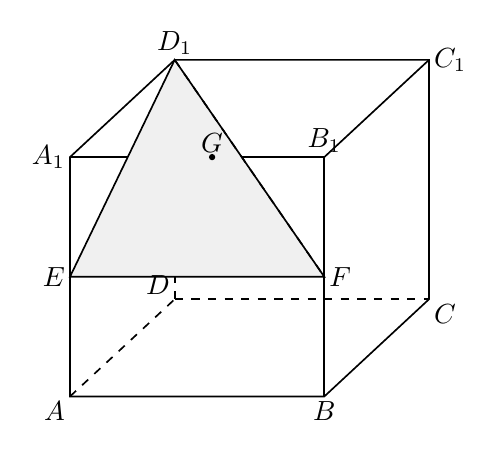
\begin{tikzpicture}[scale=0.95, semithick,
  every node/.style={inner sep=1.5pt}]
  \coordinate (A)  at (0,0);
  \coordinate (B)  at (3.4,0);
  \coordinate (C)  at (4.8,1.3);
  \coordinate (D)  at (1.4,1.3);
  \coordinate (A1) at (0,3.2);
  \coordinate (B1) at (3.4,3.2);
  \coordinate (C1) at (4.8,4.5);
  \coordinate (D1) at (1.4,4.5);
  \coordinate (E)  at (0,1.6);
  \coordinate (F)  at (3.4,1.6);
  \coordinate (G)  at (1.9,3.2);

  \draw[dashed] (A) -- (D);
  \draw[dashed] (D) -- (C);
  \draw[dashed] (D) -- (D1);
  \draw (A) -- (B) -- (C) -- (C1) -- (D1) -- (A1) -- cycle;
  \draw (A) -- (A1); \draw (B) -- (B1); \draw (C) -- (C1);
  \draw (A1) -- (B1); \draw (B1) -- (C1);
  % 平面 D1EF
  \fill[gray!12] (D1) -- (E) -- (F) -- cycle;
  \draw (D1) -- (E) -- (F) -- cycle;
  \draw[dashed] (D1) -- (F);
  \fill (G) circle (1.2pt);

  \node[below left] at (A) {$A$};
  \node[below] at (B) {$B$};
  \node[below right] at (C) {$C$};
  \node[above left] at (D) {$D$};
  \node[left] at (A1) {$A_1$};
  \node[above] at (B1) {$B_1$};
  \node[right] at (C1) {$C_1$};
  \node[above] at (D1) {$D_1$};
  \node[left] at (E) {$E$};
  \node[right] at (F) {$F$};
  \node[above] at (G) {$G$};
\end{tikzpicture}
\end{center}
\nopagebreak[4]
（A）$\sqrt3$

（B）$\dfrac{\sqrt2}{2}$

（C）$\dfrac{\sqrt2\lambda}{2}$

（D）$\dfrac{\sqrt5}{5}$

\Needspace{0.4\textheight}
\end{question}
\begin{question}
\gkti{6}为了了解某学校学生的身体发育情况，抽查了该校 $100$ 名高中男生的体重情况，根据所得数据画出样本的频率分布直方图如图所示。根据此图，估计该校 $2000$ 名高中男生中体重大于 $70.5$ 公斤的人数为（　）
\nopagebreak[4]
\begin{center}% 2007 年湖北卷文科第 6 题：100 名男生体重的频率分布直方图。
%   组距 2 kg，横轴 52.5—76.5 kg，纵轴「频率/组距」0.01—0.08。
% 来源 PDF：gaokaomath-src/普通高考/2007/2007湖北文.pdf
% SHA-256：290a153da24ec0f3a3abb8bb916d9b7e06d203d3ef5bd7bb221c93f7f1b1cacb
% 原页：2007湖北文.pdf 第 1 页（A3 三栏）第 1 栏，书页码 377。
% 重绘依据：按原页 12 个等宽柱与纵轴刻度重绘，柱高按原图读取。
\begin{tikzpicture}[x=1.0cm, y=70cm, semithick,
  every node/.style={inner sep=1pt, font=\scriptsize}]
  \draw[->,>=stealth] (0,0) -- (12.8,0) node[right] {体重 (kg)};
  \draw[->,>=stealth] (0,0) -- (0,0.09) node[above] {频率/组距};

  \foreach \i/\h in {0/0.01,1/0.01,2/0.02,3/0.05,4/0.06,5/0.07,
                     6/0.08,7/0.065,8/0.05,9/0.04,10/0.03,11/0.02} {
    \draw (\i,0) rectangle (\i+1,\h);
  }

  \foreach \y in {0.01,0.02,0.03,0.04,0.05,0.06,0.07,0.08} {
    \draw (0,\y) -- (-0.12,\y);
    \node[left] at (0,\y) {\y};
  }
  \node[below left] at (0,0) {$O$};
  \foreach \i in {1,...,12} {
    \draw (\i,0) -- (\i,-0.0015);
    \node[below] at (\i,0) {\the\numexpr 52+2*\i\relax.5};
  }
\end{tikzpicture}
\end{center}
\nopagebreak[4]
（A）$300$

（B）$360$

（C）$420$

（D）$450$

\end{question}
\begin{question}
\gkti{7}将 $5$ 本不同的书全发给 $4$ 名同学，每名同学至少有一本书的概率是（　）

（A）$\dfrac{15}{64}$

（B）$\dfrac{15}{128}$

（C）$\dfrac{24}{125}$

（D）$\dfrac{48}{125}$

\end{question}
\begin{question}
\gkti{8}由直线 $y=x+1$ 上的一点向圆 $(x-3)^2+y^2=1$ 引切线，则切线长的最小值为（　）

（A）$1$

（B）$2\sqrt2$

（C）$\sqrt7$

（D）$3$

\end{question}
\begin{question}
\gkti{9}设 $\boldsymbol a=(4,3)$，$\boldsymbol a$ 在 $\boldsymbol b$ 上的投影为 $\dfrac{5\sqrt2}{2}$，$\boldsymbol b$ 在 $x$ 轴上的投影为 $2$，且 $|\boldsymbol b|\leqslant14$，则 $\boldsymbol b$ 为（　）

（A）$(2,14)$

（B）$\left(2,-\dfrac27\right)$

（C）$\left(-2,\dfrac27\right)$

（D）$(2,8)$

\end{question}
\begin{question}
\gkti{10}已知 $p$ 是 $r$ 的充分条件而不是必要条件，$q$ 是 $r$ 的充分条件，$s$ 是 $r$ 的必要条件，$q$ 是 $s$ 的必要条件，现有下列命题：

① $s$ 是 $q$ 的充要条件；

② $p$ 是 $q$ 的充分条件而不是必要条件；

③ $r$ 是 $q$ 的必要条件而不是充分条件；

④ $\neg p$ 是 $\neg s$ 的必要条件而不是充分条件；

⑤ $r$ 是 $s$ 的充分条件而不是必要条件。

则正确命题的序号是（　）

（A）①④⑤

（B）①②④

（C）②③⑤

（D）②④⑤

\end{question}
\gkpart{二、填空题}

\begin{question}
\gkti{11}设变量 $x$，$y$ 满足约束条件 $\begin{cases}x-y+3\geqslant0,\\ x+y\geqslant0,\\ -2\leqslant x\leqslant3,\end{cases}$ 则目标函数 $2x+y$ 的最小值为\gkblank{}。

\end{question}
\begin{question}
\gkti{12}过双曲线 $\dfrac{x^2}{4}-\dfrac{y^2}{3}=1$ 左焦点 $F_1$ 的直线交双曲线的左支于 $M$，$N$ 两点，$F_2$ 为其右焦点，则 $|MF_2|+|NF_2|-|MN|$ 的值为\gkblank{}。

\end{question}
\begin{question}
\gkti{13}已知函数 $y=f(x)$ 的图象在点 $M(1,f(1))$ 处的切线方程是 $y=\dfrac12x+2$，则 $f(1)+f'(1)=$\gkblank{}。

\end{question}
\begin{question}
\gkti{14}某男运动员在三分线投球的命中率是 $\dfrac12$，他投球 $10$ 次，恰好投进 $3$ 个球的概率为\gkblank{}。（用数值作答）

\Needspace{0.4\textheight}
\end{question}
\begin{question}
\gkti{15}为了预防流感，某学校对教室用药熏消毒法进行消毒。已知药物释放过程中，室内每立方米空气中的含药量 $y$（毫克）与时间 $t$（小时）成正比；药物释放完毕后，$y$ 与 $t$ 的函数关系式为 $y=\left(\dfrac1{16}\right)^{t-a}$（$a$ 为常数），如图所示。

（1）从药物释放开始，每立方米空气中的含药量 $y$（毫克）与时间 $t$（小时）之间的函数关系式为\gkblank{}；

（2）据测定，当空气中每立方米的含药量降低到 $0.25$ 毫克以下时，学生方可进教室，那么药物释放开始，至少需要经过\gkblank{}小时后，学生才能回到教室。
\nopagebreak[4]
\begin{center}% 2007 年湖北卷文科第 15 题：药物释放过程中含药量 y 与时间 t 的关系图。
%   0—0.1 小时线性上升至 1 毫克，0.1 小时后按 (1/16)^(t-a) 衰减。
% 来源 PDF：gaokaomath-src/普通高考/2007/2007湖北文.pdf
% SHA-256：290a153da24ec0f3a3abb8bb916d9b7e06d203d3ef5bd7bb221c93f7f1b1cacb
% 原页：2007湖北文.pdf 第 1 页（A3 三栏）第 3 栏，书页码 377。
% 重绘依据：按原页折线—曲线衔接点 (0.1,1) 与衰减趋势重绘。
\begin{tikzpicture}[x=4.2cm, y=1.5cm, semithick,
  every node/.style={inner sep=1pt}]
  \draw[->,>=stealth] (0,0) -- (1.25,0) node[right] {$t$ (小时)};
  \draw[->,>=stealth] (0,0) -- (0,1.25) node[above] {$y$ (毫克)};
  \node[below left] at (0,0) {$O$};
  \draw (0,0) -- (0.1,1);
  \draw[domain=0.1:1.15,samples=100] plot (\x,{(1/16)^(\x-0.1)});
  \draw[dashed] (0.1,0) -- (0.1,1);
  \draw[dashed] (0,1) -- (0.1,1);
  \node[left] at (0,1) {$1$};
  \node[below] at (0.1,0) {$0.1$};
\end{tikzpicture}
\end{center}
\nopagebreak[4]
\end{question}
\gkpart{三、解答题}

\begin{question}
\gkti{16}已知函数 $f(x)=2\sin^2\left(\dfrac{\pi}{4}+x\right)-\sqrt3\cos2x$，$x\in\left[\dfrac{\pi}{4},\dfrac{\pi}{2}\right]$。

（1）求 $f(x)$ 的最大值和最小值；

（2）若不等式 $|f(x)-m|<2$ 在 $x\in\left[\dfrac{\pi}{4},\dfrac{\pi}{2}\right]$ 上恒成立，求实数 $m$ 的取值范围。

\Needspace{0.4\textheight}
\end{question}
\begin{question}
\gkti{17}如图，在三棱锥 $V-ABC$ 中，$VC\perp$ 底面 $ABC$，$AC\perp BC$，$D$ 是 $AB$ 的中点，且 $AC=BC=a$，$\angle VDC=\theta$（$0<\theta<\dfrac{\pi}{2}$）。

（1）求证：平面 $VAB\perp$ 平面 $VCD$；

（2）试确定角 $\theta$ 的值，使得直线 $BC$ 与平面 $VAB$ 所成的角为 $\dfrac{\pi}{6}$。
\nopagebreak[4]
\begin{center}% 2007 年湖北卷文科第 17 题：三棱锥 V-ABC，VC⊥底面 ABC，D 为 AB 中点。
% 来源 PDF：gaokaomath-src/普通高考/2007/2007湖北文.pdf
% SHA-256：290a153da24ec0f3a3abb8bb916d9b7e06d203d3ef5bd7bb221c93f7f1b1cacb
% 原页：2007湖北文.pdf 第 2 页（A3 三栏）第 3 栏，书页码 378。
% 重绘依据：按原页 V、A、B、C、D 的位置与虚线重绘。
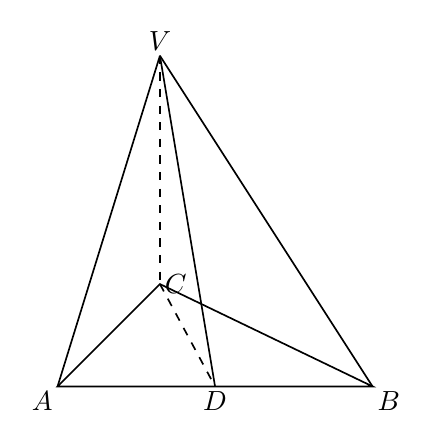
\begin{tikzpicture}[scale=1.0, semithick,
  every node/.style={inner sep=1.5pt}]
  \coordinate (A) at (0,0);
  \coordinate (B) at (4.0,0);
  \coordinate (C) at (1.3,1.3);
  \coordinate (V) at (1.3,4.2);
  \coordinate (D) at (2.0,0);

  \draw (A) -- (B) -- (C) -- cycle;
  \draw (V) -- (A);
  \draw (V) -- (B);
  \draw[dashed] (V) -- (C);
  \draw (V) -- (D);
  \draw[dashed] (C) -- (D);

  \node[below left] at (A) {$A$};
  \node[below right] at (B) {$B$};
  \node[right] at (C) {$C$};
  \node[above] at (V) {$V$};
  \node[below] at (D) {$D$};
\end{tikzpicture}
\end{center}
\nopagebreak[4]
\end{question}
\begin{question}
\gkti{18}某商品每件成本 $9$ 元，售价 $30$ 元，每星期卖出 $432$ 件。如果降低价格，销售量可以增加，且每星期多卖出的商品件数与商品单价的降低值 $x$（单位：元，$0\leqslant x\leqslant30$）的平方成正比。已知商品单价降低 $2$ 元时，一星期多卖出 $24$ 件。

（1）将一个星期的商品销售利润表示成 $x$ 的函数；

（2）如何定价才能使一个星期的商品销售利润最大？

\end{question}
\begin{question}
\gkti{19}设二次函数 $f(x)=x^2+ax+a$，方程 $f(x)-x=0$ 的两根 $x_1$ 和 $x_2$ 满足 $0<x_1<x_2<1$。

（1）求实数 $a$ 的取值范围；

（2）试比较 $f(0)f(1)-f(0)$ 与 $\dfrac1{16}$ 的大小，并说明理由。

\end{question}
\begin{question}
\gkti{20}已知数列 $\{a_n\}$ 和 $\{b_n\}$ 满足：$a_1=1$，$a_2=2$，$a_n>0$，$b_n=\sqrt{a_na_{n+1}}$（$n\in\mathbf N^*$），且 $\{b_n\}$ 是以 $q$ 为公比的等比数列。

（1）证明：$a_{n+2}=a_nq^2$；

（2）若 $c_n=a_{2n-1}+2a_{2n}$，证明数列 $\{c_n\}$ 是等比数列；

（3）求和：$\dfrac1{a_1}+\dfrac1{a_2}+\dfrac1{a_3}+\dfrac1{a_4}+\cdots+\dfrac1{a_{2n-1}}+\dfrac1{a_{2n}}$。

\Needspace{0.4\textheight}
\end{question}
\begin{question}
\gkti{21}在平面直角坐标系 $xOy$ 中，过定点 $C(0,p)$ 作直线与抛物线 $x^2=2py$（$p>0$）相交于 $A$，$B$ 两点。

（1）若点 $N$ 是点 $C$ 关于坐标原点 $O$ 的对称点，求 $\triangle ANB$ 面积的最小值；

（2）是否存在垂直于 $y$ 轴的直线 $l$，使得 $l$ 被以 $AC$ 为直径的圆截得的弦长恒为定值？若存在，求出 $l$ 的方程；若不存在，说明理由。
\nopagebreak[4]
\begin{center}% 2007 年湖北卷文科第 21 题：抛物线 x^2=2py，过 C(0,p) 的直线交于 A、B，
%   N 为 C 关于原点的对称点。
% 来源 PDF：gaokaomath-src/普通高考/2007/2007湖北文.pdf
% SHA-256：290a153da24ec0f3a3abb8bb916d9b7e06d203d3ef5bd7bb221c93f7f1b1cacb
% 原页：2007湖北文.pdf 第 2 页（A3 三栏）第 3 栏，书页码 378。
% 重绘依据：按原页抛物线、割线与 C、N 的位置重绘，p=1 仅作示意。
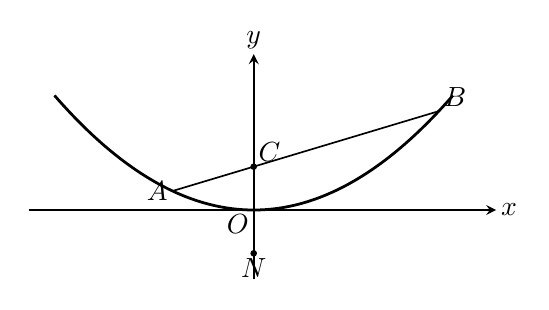
\begin{tikzpicture}[x=1.1cm, y=0.55cm, semithick,
  every node/.style={inner sep=1.5pt}]
  \draw[->,>=stealth] (-2.6,0) -- (2.8,0) node[right] {$x$};
  \draw[->,>=stealth] (0,-1.6) -- (0,3.6) node[above] {$y$};
  \node[below left] at (0,0) {$O$};

  \draw[domain=-2.3:2.3,samples=120,line width=1pt] plot (\x,{\x*\x/2});

  \coordinate (C) at (0,1);
  \coordinate (N) at (0,-1);
  \coordinate (A) at (-0.937,0.439);
  \coordinate (B) at (2.137,2.283);

  \draw (A) -- (B);
  \fill (C) circle (1.2pt);
  \fill (N) circle (1.2pt);
  \node[above right] at (C) {$C$};
  \node[below] at (N) {$N$};
  \node[left] at (A) {$A$};
  \node[above right] at (B) {$B$};
\end{tikzpicture}
\end{center}
\nopagebreak[4]

\end{question}